%\chapter{det-comp}


%%%%%%%%%%%%%%%%%%%%%%%%%%%%%%%%%%%%%%%%%%%%%%
%\section{Anode Plane Assemblies}

%%%%%%%%%%%%%%%%%%%%%%%%%%%%%%%%%%%%%%%%%%%%%%
%\section{Cathode Plane Assemblies}

%%%%%%%%%%%%%%%%%%%%%%%%%%%%%%%%%%%%%%%%%%%%%%
%\section{Field Cage}

%%%%%%%%%%%%%%%%%%%%%%%%%%%%%%%%%%%%%%%%%%%%%%
%\section{HV components}

%%%%%%%%%%%%%%%%%%%%%%%%%%%%%%%%%%%%%%%%%%%%%%
%\section{TPC front-end electronics and DAQ}

%%%%%%%%%%%%%%%%%%%%%%%%%%%%%%%%%%%%%%%%%%%%%%
%\section{PDS front-end electronics and DAQ}

%%%%%%%%%%%%%%%%%%%%%%%%%%%%%%%%%%%%%%%%%%%%%%
%\section{Cryostat and feedthroughs}

%%%%%%%%%%%%%%%%%%%%%%%%%%%%%%%%%%%%%%%%%%%%%%
%\section{Cryostat and LAr purification system}

%%%%%%%%%%%%%%%%%%%%%%%%%%%%%%%%%%%%%%%%%%%%%%

\section{Detector monitoring and slow control}
\label{sec:slowcontrol}
The scope of the ProtoDUNE detector control system includes the design, procurement, fabrication, testing,
delivery, installation oversight and acceptance tests of a comprehensive detector monitoring, control and safety system,
fulfilling the needs of the protoDUNE detectors and experiment's infrastructure.

The responsibility for the system is split into two main blocks: All the devices that will be installed and cabled inside 
the cryostat, the sensors needed to monitor the cryostat itself as well as the specification of the system needs is a 
responsibility of the protoDUNE collaboration; the implementation of the control system (hardware, firmware and sw) outside 
the cryostat will be taken care of by CERN. Together, these two blocks form the overall detector control system and is the 
responsibility of the slow control group.

In this section the main system requirements will be described in terms of constraints, assumptions and functional 
requirements; the sensors, power supplies, etc. foreseen for protoDUNE will be detailed out; and the general structure of 
the control system will be described.


\subsection{Constraints and requirements}
\begin{enumerate}
\item	The control and safety system for SP protoDUNE shall be based on the experience gained, the design developed and the 
components chosen for the 3mx1mx1m WA105 DP protoDUNE prototype.
\item	The control and safety system for SP protoDUNE shall be prepared, commissioned and installed on the timescales 
required by the experiment.

\item	The physical interface of the system taken care of by CERN is at the level of the outer flanges on the cryostat. 
Sensors, power distribution, etc. inside the cryostat are part of the experiment's responsibilities, while CERN will take 
care of connecting the control system to the flanges.
\item	The slow control group is not responsible for the site and peripheral infrastructure (cables, patch panels, 
platforms, safety items, Power 400V, UPS, etc.).
\item	The system specification (I/O parameters, control \& safety logics, etc.) is provided by the SP protoDUNE 
collaboration.
\item	The system developed by CERN will interface to the cryogenic control infrastructure for information and signal 
exchanges. 
\item	The final test and commissioning in building 887 (EHN1, Prevessin) will be carried out jointly by the SP protoDUNE 
collaboration and EP/DT-DI.
\item	A person from the SP protoDUNE collaboration will work side by side with CERN to contribute to the SCADA 
supervisor and user interface developments and ensure regular information exchange.

\item	CERN shall design, procure components, construct and test the control and safety system according to the SP protoDUNE specifications.
\item	CERN shall develop and test the SCADA supervisor for SP protoDUNE.
\item	CERN shall deliver a complete set of technical documentation, comprising technical drawings, hardware components lists, installation and commissioning instructions, operations instructions and hand-over documents.
\item	CERN shall participate to the final test and commissioning of the system in building 887 (EHN1, Prevessin).
\item	The Process Control System shall do the reading of temperature sensors, pressure sensors, trace analysers (O2, N2, H2O).
\item	The Detector Control System shall monitor and control the LV and HV.
\item	The Detector Safety System shall ensure the safety of the experiment.
\item	The Detector Safety System shall perform the temperature survey.
\item	The Detector Safety System shall take care of interlocks.
\item	The system shall provide a graphical user interface to visualize the trends of monitored values, the alarms, as well as to control the experiment.
\item	The system should provide a web interface to be able to remotely monitor the behaviour of the experiment.
\end{enumerate}
\subsection{Devices}
Add here PMT \& TPC (HV, LV, current monitors?), temperature and pressure sensors, level meters?, camera vision inside tank?, trace analysers, 
calibration system?,... 

\subsection{General layout of the detector control and safety system}
The design of the protoDUNE SP control system is based on the experience gained in collaboration with ETH Zurich during a pilot (WA105) project 
aimed at validating, among others, the design of the control system for such types of detectors. 

Figure XX shows the general architecture of the control and safety system for protoDUNE.
The system is subdivided into the Process Control System, the Detector Control System and the Detector Safety System. For the DP protoDUNE detector an additional element is included for the motorization of the Charge Readout Plane (CRP).

\begin{cdrfigure}[DCS design]{dcsdesign}{Proposed architecture and technical solution of the control and safety system.}
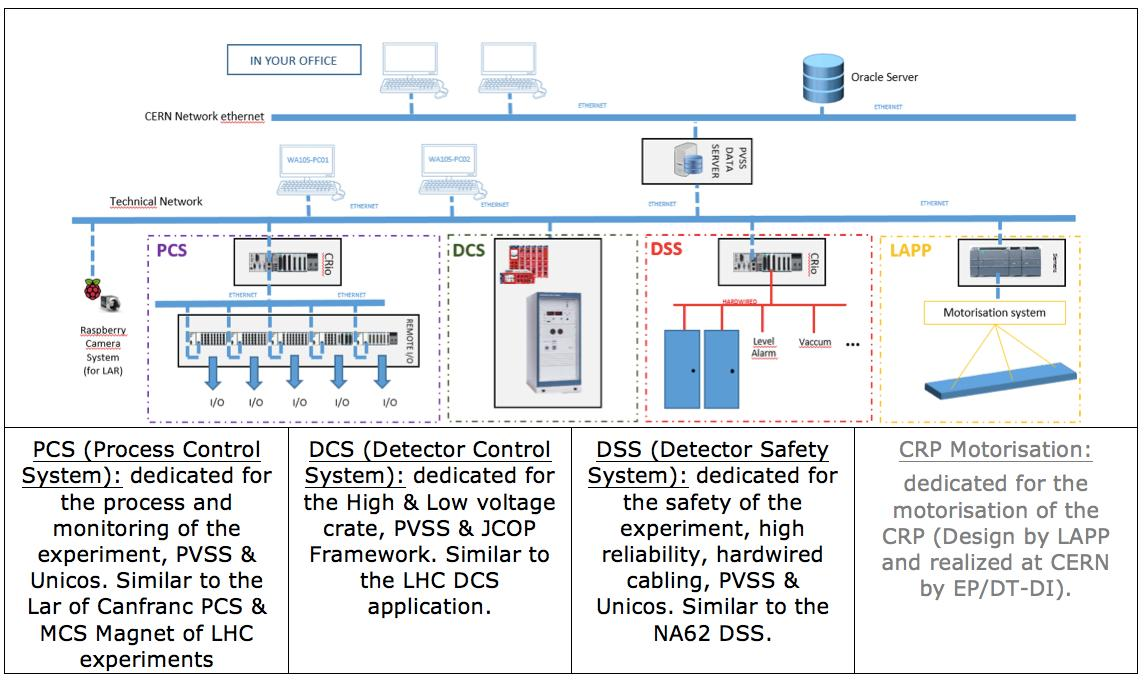
\includegraphics[width=0.8\textwidth, angle=90]{DCS_Design}
\end{cdrfigure}

The control system for each detector will be composed of the following elements:
\begin{enumerate}
\item	A chassis for electrical distribution (380Vac, 220Vac, 24Vdc redundant).
\item	Two chassis for PCS (Process Control System) composed of an FPGA, signal conditioners, interface, and cabling.
\item	One chassis for DCS (Detector Control System) composed of an interface for LV/HV monitoring \& control.
\item	A chassis for DSS (Detector Safety System) composed of an FPGA and relays for the safety of the experiment.
\item	A chassis for a PC data acquisition \& supervision (PVSS SCADA Supervisor) composed of a computer with a display monitor, a switch and a 
server.
\item	Four chassis for the remote I/O to capture signal close to the detector and avoid multi-cabling structure.
\item	One chassis for HV controlled by the slow control system.
\end{enumerate}
All these elements, will be mounted in the 19-in. racks (see Figure Y).
\begin{cdrfigure}[DCS racks]{dcsracks}{Proposed racks layout of the control and safety system.}
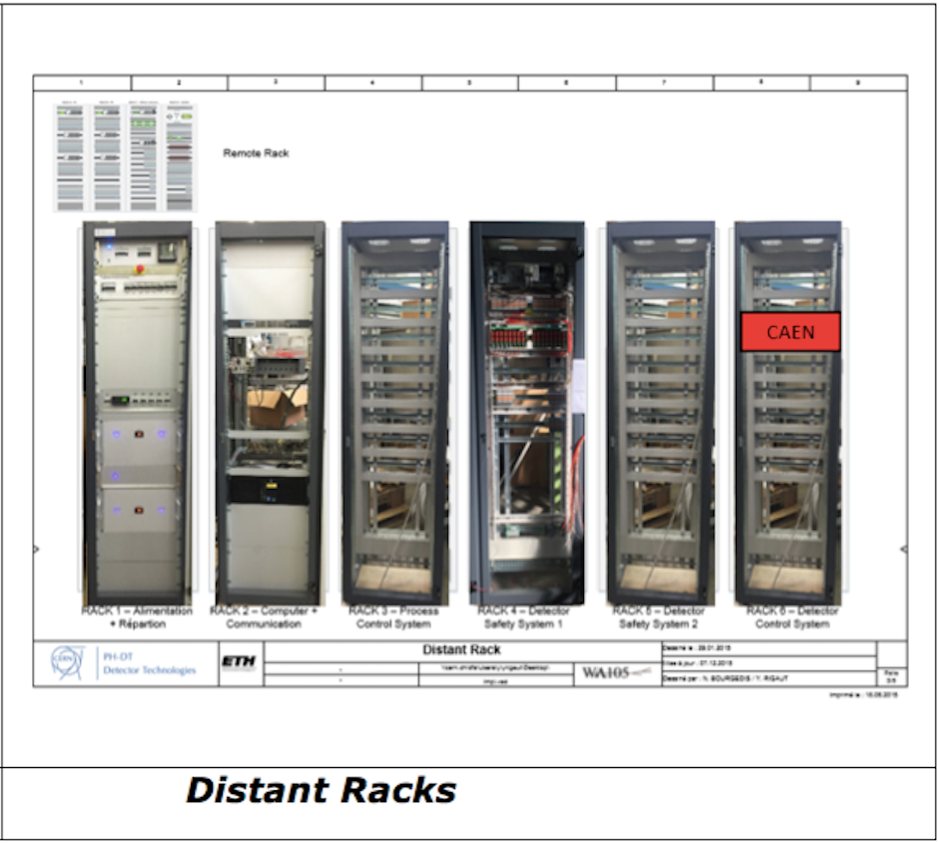
\includegraphics[width=0.8\textwidth, angle=90]{DCS-distant-racks}
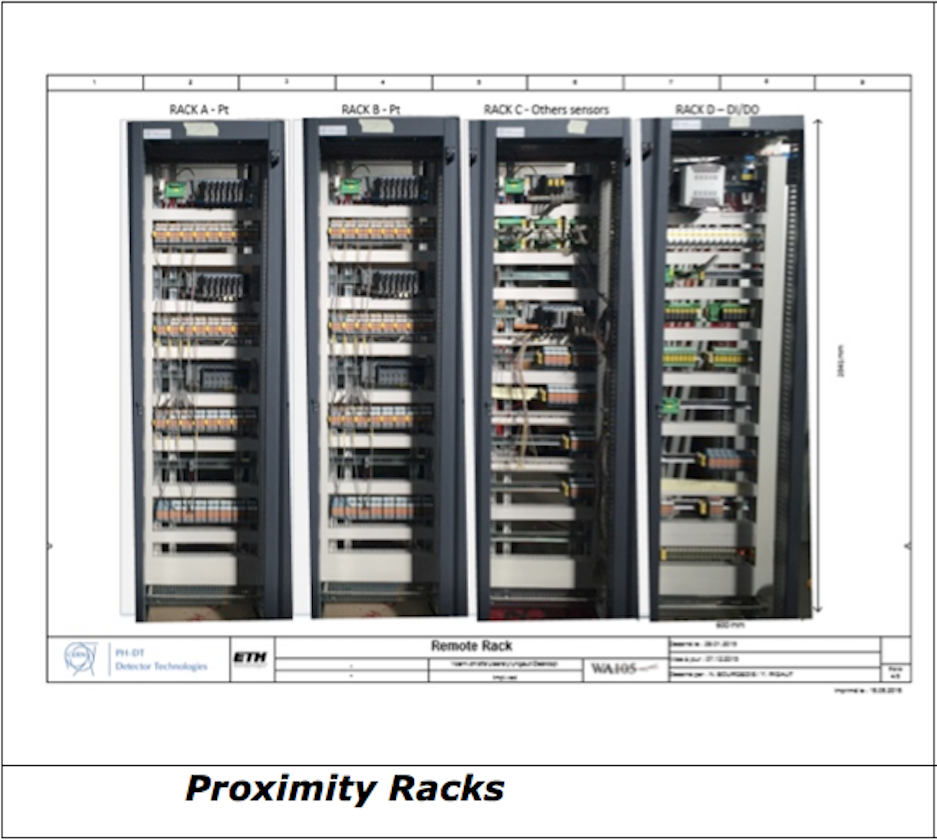
\includegraphics[width=0.8\textwidth, angle=90]{DCS-proximity-racks}
\end{cdrfigure}

The supervisory software will by based on the JCOP framework \fixme{(add ref.)}, originally developed for the LHC experiments at CERN and now used in several more experiments at CERN. Besides providing a supervisory control and data acquisition system, the framework offers many tools for the implementation of finite state machines, archival of data, as well as graphical interfaces as web dashboards.

%%%%%%%%%%%%%%%%%%%%%%%%%
\subsection{QC Procedures}
